\rhead{OUTILS}

\lettrine[lines=2,slope=0pt,nindent=4pt]{\textbf{T}}{rioCFD} dispose de deux Trackers sous l'outil TULEAP \cite{TULEAP}. Ils ont tous deux des utilit\'es diff\'erentes
l'un \'etant d\'edi\'e \`a la gestion du code (Demandes d'Intervention, D\'eveloppements, Bugs,...) tandis que l'autre constitue un outil de suivi et d'archivage des \'etudes effectu\'ees sous TrioCFD. Par cons\'equent, leur constitution et leur utilisation sont totalement diff\'erentes et vont \^etre d\'etaill\'ees dans les deux premiers chapitres de cette partie. Nous nous int\'eresserons ensuite \`a l'outil de gestion du code (GIT) puis, les diff\'erentes messageries du projet pour finir par une cartographie des diff\'erents outils d'interfa\c cage.

\chapter{\label{chapitre:tracker-info}Tracker informatique - TULEAP}
\lhead{Tracker informatique - TULEAP}
\rhead{OUTILS}

Le code TrioCFD dispose d'un projet propre sous TULEAP accessible à l'adresse \url{https://codev-tuleap.intra.cea.fr/projects/triocfd/}.
Il a pour but de r\'epertorier l'ensemble des actions de correction, d\'eveloppement, assistance et livraison men\'ees sur le code.

\subsection{Constitution du projet TrioCFD}

Dans ce projet TULEAP, diff\'erents outils sont disponibles via le bandeau de gauche : \newline
\begin{itemize}[label=$\Rightarrow$, font=\LARGE]
   \item \textbf{TrioCFD BugTracker} : outil de trackage des diff\'erents d\'eveloppements, correctifs, demandes d'assis\-tance,... qui concernent le code TrioCFD. Chaque fiche dispose d'un seul et unique num\'ero d'identification qui est utilis\'e pour la d\'enomination des branches du gestionnaire de contr\^ole des versions, GIT. Cet outil, assez cons\'equent est d\'ecrit plus en d\'etail par la suite.
   \begin{multicols}{2} 
   \item \textbf{Documents} : regroupe les diff\'erents documents \`a destination des utilisateurs CEA de TrioCFD (archivage des pr\'esentations des s\'eminaires, des notes techniques CEA, des sp\'ecifications techniques...). La structure est illustrée sur la figure \ref{figure:tuleap_doc}.
   \columnbreak 
   \begin{center}
   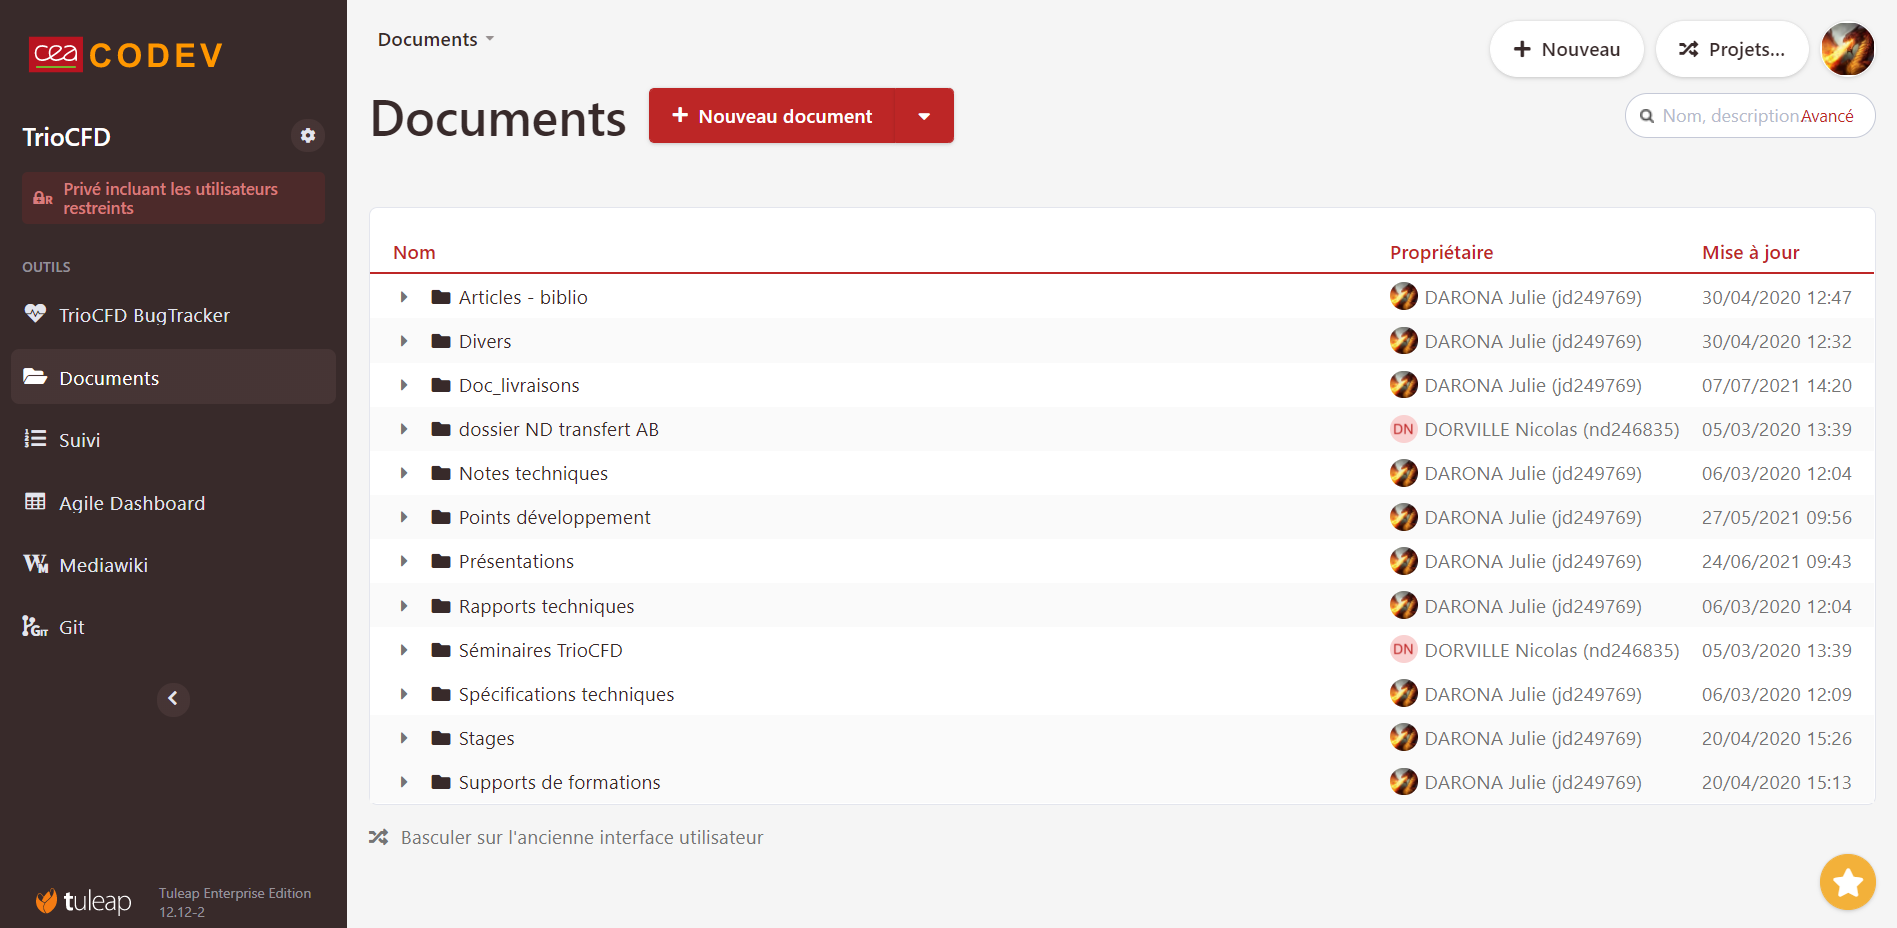
\includegraphics[width=7cm]{pictures/tuleap_documents.png}
   \captionof{figure}{\label{figure:tuleap_doc}Structure de la base documentaire sur TULEAP}
   \end{center}
   \end{multicols}
   \item \textbf{Agile Dashboard} : outil de planification des int\'egrations en vue des livraisons du code. Cet outil a commenc\'e \`a \^etre mis en place \`a partir de la version v1.8.1 (juin 2020). Son utilisation n'est pas encore optimale mais monte progressivement en puissance.
   \item \textbf{MediaWiki} : outil d'aide \`a destination des d\'eveloppeurs pour l'installation de leur environnement de travail
   \newpage
   \item \textbf{Git} : le syst\`eme de contr\^ole des versions sous base GIT est heberg\'e sous TULEAP et est accessible ici. On y trouve  l'adresse du d\'ep\^ot n\'ecessaire pour faire le clonage (voir figure \ref{figure:tuleap_clone}). Aucune action GIT ne doit \^etre lanc\'ee depuis TULEAP car source de nombreuses erreurs. Seules les Pull Request sont effectu\'ees depuis TULEAP en choisissant, dans les menus d\'eroulants, d'une part la branche voulant \^etre int\'egr\'ee et d'autre part, la branche recevant l'int\'egration (voir figure \ref{figure:tuleap_PR}).
   \begin{multicols}{2}
   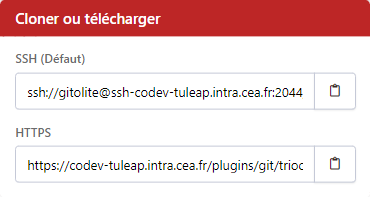
\includegraphics[width=7cm]{pictures/Tuleap_clone.png}
   \captionof{figure}{\label{figure:tuleap_clone}R\'ecup\'eration de l'adresse du d\'ep\^ot GIT via TULEAP}
   \columnbreak
   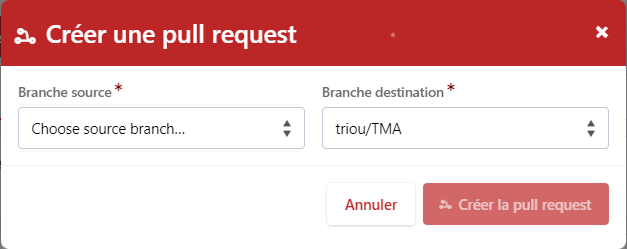
\includegraphics[width=7cm]{pictures/PR.png}\vspace*{1.1cm}
   \captionof{figure}{\label{figure:tuleap_PR}Création d'une Pull Request depuis Tuleap}
   \end{multicols}
\end{itemize}

Nous allons maintenant d\'etailler la partie BugTracker du projet TULEAP de TrioCFD.
\subsection{Fonctionnement g\'en\'eral du BugTracker informatique}
Le BugTracker informatique est utilisé autant par l'\'equipe de TMA que par les agents CEA. A chaque action concernant le code, une fiche spécifique est créée (fiche de Demande d'Intervention). Les fiches répertoriées sur le BugTracker peuvent \^etre trait\'ees soit par l'équipe TMA soit par l'équipe CEA suivant la nature de la fiche. La répartition du traitement des fiches est gérée par le Responsable de Code via le champs \texttt{Way of treatment} de chaque fiche.\\

Pour les demandes re\c cues sur les adresses \'electroniques du projet (voir Chapitre \ref{chapitre:messagerie}), les fiches sont exclusivement ouvertes par l'\'equipe TMA. En revanche, pour les fiches attribu\'ees \`a l'\'equipe CEA, celles-ci sont ouvertes soit directement par un membre de l'\'equipe soit par le responsable de code.\\

Afin de garantir une bonne traçabilité, chaque action de modification, correction ou évolution faite dans le code nécessite l'ouverture au préalable, d'une fiche de Demande d'Intervention. A chaque fiche d'intervention, correspond une branche de développement spécifique dans le gestionnaire de versions dont le nom inclut l'identifiant de la fiche. Ainsi, à tout moment, il est possible de connaître la raison du mouvement des sources du code mais également de connaître l'influence de ce mouvement sur la validation. Nous reviendrons, par la suite, plus en détails sur ces aspects de traçabilité.\\

\subsection{\label{subsec: ficheDI}Constitution d'une fiche de demande d'intervention}
Une fiche de demande d'intervention est constituée de multiples champs. Tous ne sont pas syst\'ematiquement d\'efinis mais les champs vivement recommandés sont détaillés ci-après :\\
\begin{itemize}[label=$\Rightarrow$, font=\LARGE]
   \item \textbf{liste\_diffusion} (\textit{type :} liste ouverte avec lien vers les membres du projet) : permet de retrouver, dans l'annuaire du BugTracker, les personnes potentiellement intéressées/concernées par la fiche. Toute personne identifiée dans ce champ recevra un e-mail automatique du BugTracker la renseignant sur les modifications apportées dans la fiche.
   \item \textbf{Summary} (\textit{type :} chaîne de caractère - \textbf{champ obligatoire}) : correspond au titre de la Demande d'Intervention. Celui-ci doit être court tout en identifiant clairement le problème constaté.  
   \item \textbf{Original Submission} (\textit{type :} Texte) : décrit en détails le problème rencontré ou le développement prévu. Comme, il s'agit d'un champ sans restriction, il est recommandé de donner le maximum d'informations sur le contexte de la fiche et les attendus.
   \item \textbf{Priority} (\textit{type :} liste de choix) : définit la priorité de la fiche considérée par rapport aux autres ouvertes. Ce champ est principalement à destination de l'équipe TMA afin qu'elle soit renseignée sur la priorité de traitement des fiches en fonction des contraintes projet. L'affectation a une priorité induit un délai de résolution : 1-High -> 10 jours ouvrés ; 2-Medium -> 22 jours ouvrés ; 3-Low -> avant la prochaine livraison de version. Le compteur débute à la date renseignée dans le champs \textit{Date hiérarchisation}.
   \item \textbf{Category} (\textit{type :} liste de choix) : correspond à une des catégories de Demandes d'Intervention listées au Chapitre \ref{chapitre:termes} et identifiées dans le contrat de marché de la TMA.
   \item \textbf{Sub project associated} (\textit{type :} liste de choix) : permet d'identifier le module impacté par la DI.
   \item \textbf{Authorization to work on this} (\textit{type :} case à cocher) : champ destiné à la TMA pour lui donner l'autorisation de débuter les travaux sur la DI.
   \item \textbf{Date hiérarchisation} (\textit{type :} date) : champ à mettre à jour avec le champ précédent (Authorization to work on this) et à renseigner avec la date du jour du lancement des travaux sur la DI. Cette date permettra de vérifier que le délai de réalisation de la DI est bien tenu.
   \item \textbf{Status} (\textit{type :} liste de choix) : correspond à l'état de vie de la fiche. Cette notion sera plus approfondie dans la section suivante (voir section \ref{sec:etatsDI}). 
   \item \textbf{Assigned to} (\textit{type :} liste à choix multiples avec lien vers les membres du projet) : correspond à(aux) membre(s) du projet travaillant sur le traitement de la DI.
   \item \textbf{Way of treatment} (\textit{type :} liste de choix) : 2 choix sont possibles ; soit la demande est traitée par le CEA (\textit{ResolutionByCEA}) soit par la TMA (\textit{ResolutionByTMA}).
   \item \textbf{Work load} (\textit{type :} flottant) : champ renseigné uniquement lorsque la DI est traitée par l'équipe TMA afin de s'assurer que la charge de traitement n'a pas été trop conséquente et a bien respecté les indicateurs contractuels.
\end{itemize}

%\begin{multicols}{2}
\begin{minipage}[c]{0.35\linewidth}

\vspace*{0.2cm}
Ainsi, l'aspect général de la fiche au moment de sa création est visualisable ci-contre (voir Figure \ref{figure:fiche_DI})
\\
Tous les champs ne sont pas obligatoires à la création de la fiche mais peuvent le devenir en fonction de son état de traitement. De même, tous les champs sont modifiables à tout moment. Ainsi, on veillera à mettre à jour le titre de la fiche si, lors de son traitement, on constate que le problème avait été initialement mal identifié.\\
\\
\\
La gestion du BugTracker Tuleap est du ressort du Responsable de Code. En fonction de l'évolution des besoins, des adaptations de ces champs pourront ponctuellement être faites.
\\
\\
\end{minipage} \hfill
\begin{minipage}[c]{0.6\linewidth}
   
   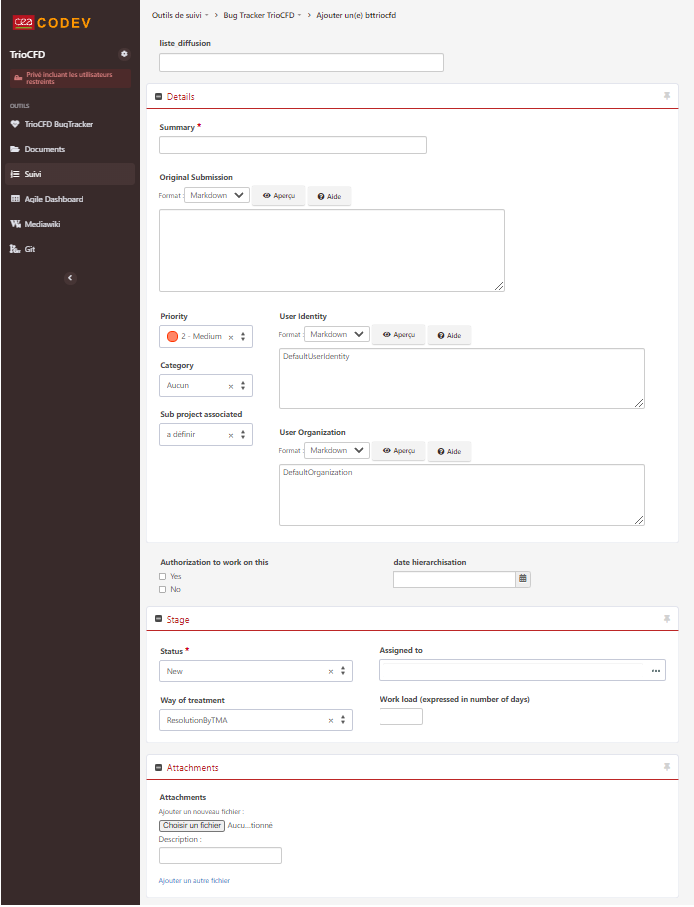
\includegraphics[width=9.5cm]{pictures/Fiche_DI.png}\vspace*{0.2cm}
   \captionof{figure}{\label{figure:fiche_DI}Champs à renseigner pour la création d'une Demande d'Intervention TrioCFD}
%\end{multicols}
\end{minipage}

Une fois la fiche de DI créée, celle-ci est répertoriée dans le BugTracker avec un identifiant unique à 6 chiffres qui servira à nommer la branche GIT associée. On observera sur la figure \ref{figure:tracker_overview}, cet identifiant dans la $1^{ère}$ colonne du tableau.\\ \vspace*{0.3cm}

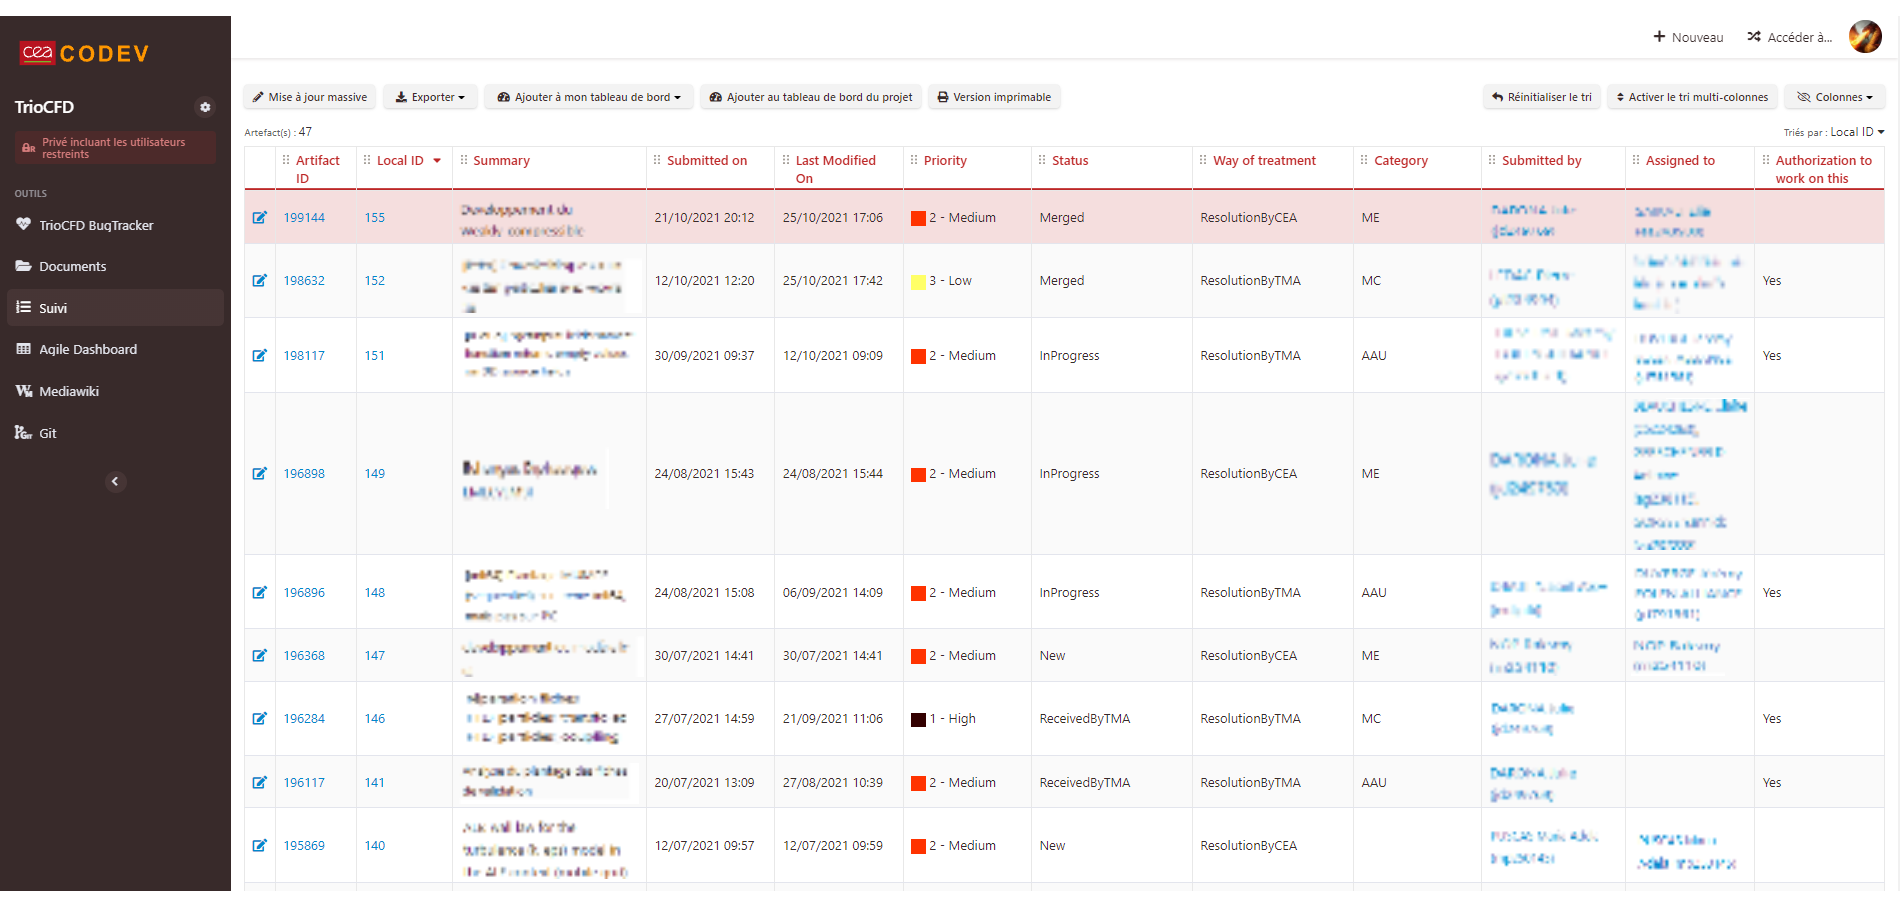
\includegraphics[width=16cm]{pictures/tracker_overview.png}\vspace*{0.1cm}
\captionof{figure}{\label{figure:tracker_overview} Vue générale du BugTracker TrioCFD et de quelques fiches de Demandes D'Intervention en cours}
\vspace*{0.3cm}
La vue générale de la figure \ref{figure:tracker_overview} permet d'avoir rapidement la visualisation des fiches ouvertes, leur priorité, leur état d'avancement et les personnes en charge de leur résolution. Cette vue peut être ajustée en fonction des besoins de suivi et ses différentes configurations, conservées.

\subsection{\label{sec:etatsDI}États de traitement d'une fiche de Demande d'Intervention }
Une fiche de DI du BugTracker TrioCFD suit un processus de traitement clairement défini et a, suivant son état, un statut particulier défini dans le champ \texttt{Status}. Ce cycle de vie est illustré par la figure \ref{figure:workflow_Trio}. Il est composé de 6 états (dans les boites rectangulaires) qui sont :\newline
\begin{itemize}[label=$\Rightarrow$, font=\LARGE]
   \item \textbf{NEW} : pour une DI saisie directement par l'utilisateur (agent CEA), une fois les champs précisés au paragraphe précédent, remplis et la création de la fiche validée, celle-ci passe automatique en statut NEW.
   \item \textbf{RECEIVED BY TMA} : (pour une DI créée par l'équipe TMA) une fois les champs précisés au paragraphe précédent remplis et la création de la fiche validée, la TMA la définit en statut RECEIVED BY TMA. Il en est de même pour les DI en statut NEW lorsque son traitement est du ressort de la TMA. Cet état signifie que la TMA a menée une première analyse de la demande et a commencé à identifier l'origine du problème. Ces premiers résultats d'analyse seront discutés lors de la réunion hebdomadaire entre le RPL et le RML. Il sera alors décidé de la pertinence de cette demande, de sa priorité de traitement (champ \texttt{Priority)} et du lancement ou non des travaux sur celle-ci (champ \textit{Authorization to work on this}).
   \item \textbf{IN PROGRESS} : lorsque le traitement d'une fiche débute, il appartient à la personne en charge de son traitement de la passer en statut IN PROGRESS. Ce changement de statut nécessite de renseigner le champ \texttt{Assigned to} afin qu'il soit pris en compte. Cet état permet de savoir que les travaux ont débuté sur le sujet. C'est dans ce statut que la DI passera la plus grande partie de sa vie. Lorsque le travail sera achevé, si la DI nécessite une modification du code source, une Pull Request (voir figure \ref{figure:tuleap_PR}) sera effectuée par la personne ayant traitée la DI.
   \item \textbf{MERGED} : une fois la branche correspondante à la DI intégrée dans la branche de développement du code (branche \texttt{triou/TMA}) par l'Intégrateur, celui-ci la passe en statut MERGED. L'équipe de TMA aura ainsi connaissance des intégrations d'un jour sur l'autre et prêtera une attention toute particulière au retour hebdomadaire de l'atelier de Vérification. En cas d'impacts non attendus sur la base de vérification, la DI est repassée en statut IN PROGRESS afin d'investiguer sur ces écarts imprévus et les justifier ou apporter des correctifs pour les résorber. Ce statut concerne uniquement les DI de type MC (Maintenance Corrective) ou de type ME (Maintenance Évolutive). 
   \item \textbf{TREATED/RESOLVED} : cet état signifie que l'ensemble des travaux nécessaires pour mener à bien le traitement de la fiche ont été faits. Dans le cas d'une ME ou d'une MC, ce statut est atteint lorsque la branche de travail a été intégrée avec succès dans la branche en développement du code et que les éventuels impacts ont été validés. Pour une fiche de type AAU, l'initiateur de la demande a retourné un avis positif sur la solution proposée pour résoudre son problème.
   \item \textbf{CLOSED} : le travail réalisé dans le cadre de cette Demande d'Intervention est validé par le RPL (demandes en traitement TMA) ou par le Responsable de Code (demandes en traitement CEA). Une fois cet état atteint, plus aucun travail ne doit être mené sur la demande. Si d'aventure, d'avantage de travail était identifié à posteriori, une nouvelle fiche devra alors être créée. 
\end{itemize}
\vspace*{0.5cm}
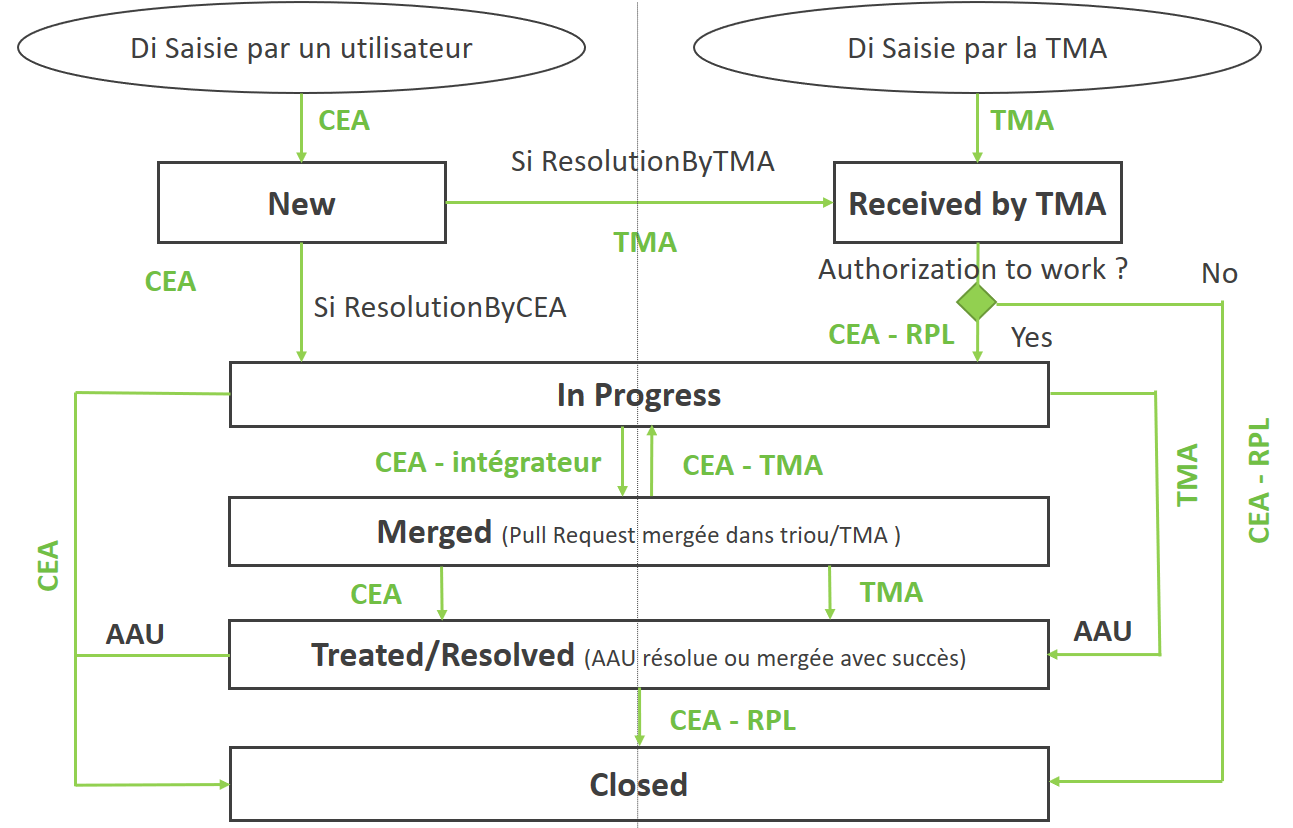
\includegraphics[width=16cm]{pictures/workflow_Trio.png}\vspace*{0.1cm}
\captionof{figure}{\label{figure:workflow_Trio} Workflow du BugTracker TrioCFD}
\vspace*{1.5cm}
L'ensemble de cette démarche est également expliquée dans le MediaWiki du BugTracker TrioCFD. \\
\\ Le respect de ces procédures garantit une bonne tra\c cabilité de l'ensemble des actions relatives au code mais également de toute modification apportée dans les sources. Le Responsable de Code a donc pour mission des les expliquer et de veiller à leur bonne application. En cas de non respect, il a à sa charge d'apporter les modifications nécessaires afin de rétablir leur bon déroulement (saisie des fiches de DI, rappel à l'ordre, blocage provisoire des droits d'intégration,...).

\newpage
\chapter{Suivi et archivage des études}
\lhead{Suivi et archivage des études}
\rhead{OUTILS}
Pour le suivi et l'archivage des études menées sous TrioCFD, le code dispose d'un Tracker propre sous Tuleap dans le projet Etudes-STMF à l'adresse : \url{https://codev-tuleap.intra.cea.fr/projects/etudes-stmf/}. D'autres codes du service sont également hébergés sous ce projet Tuleap mais chacun d'eux dispose de son propre Tracker. Si quelques adaptations sont nécessaires d'un code à l'autre pour répondre au mieux à leurs besoins, ils restent néanmoins très proches afin d'en faciliter la consultation. Ce projet a été mis en place début 2019 et est rentré en production mi 2019. Le Tracker de chacun des codes permet d'assurer un suivi de chacune des études menées sur le code concerné. Il n'est en aucun cas un lieu d'archivage des études. Pour l'archivage, un espace dédié a été créé sur le nouveau système de stockage Linux du service nommé TITANIA. Le lien avec cet espace de stockage ainsi que sa structure seront détaillés dans la dernière section de ce chapitre.
\subsection{Objectifs du suivi et de l'archivage des études}
Avant la création de ce système, aucun outil n'était proposé pour conserver une mémoire de l'ensemble des études menées sur un code. Chacun conservait, en local sur son poste de travail, les études qu'il avait réalisées. Or cette méthodologie de travail présente de forts inconvénients et risques parmi lesquels, on peut citer : 
\begin{itemize}
   \item Pertes scientifiques très conséquentes en cas de départ de la personne ayant réalisé des études sur un code ou en cas de changement de localisation des activités
   \item Pas de "mémoire" des codes sur les études pour lesquelles ils ont été utilisés
   \item Anciennes études inexploitables au fur à mesure que le temps passe
   \item Incapacité de reproductibilité des dossiers de sureté
   \item Limitations de la mutualisation des connaissances (échanges sur les pistes suivies ayant abouti ou non à la résolution des problèmes, avis des développeurs pouvant aider la partie étude,…)
   \item Benchmark entre les différents codes peu nombreux
   \item Couplage entre les différents codes peu nombreux
   \item Doublement d'études en cas de manque de dialogue entre les projets ou les laboratoires
   \item Pas de réelle vision d'ensemble de la multitude des actions menées dans le service
\end{itemize}
Les objectifs de ce suivi sont donc de limiter autant que possible les problèmes identifiés précédemment.

\subsection{Constitution d'une fiche de Suivi d'Etude}
Comme les fiches de Demande d'Intervention, les fiches de Suivi d'Etude contiennent plusieurs champs. Ils sont moins nombreux que ceux d'une Demande d'Intervention informatique car ce Tracker ne s'adresse pas au même public et son utilisation se doit d'être plus simple.  Une fiche de Suivi d'Etude est constituée de plusieurs rubriques, chacune étant constituée de différents champs. L'ensemble de cette structure est détaillée ci-dessous.\\
\begin{minipage}[c]{0.45\linewidth}
\textbf{Général}

\begin{itemize}[label=$\Rightarrow$, font=\LARGE]
   \item \textbf{Titre de l'étude} (\textit{type :} chaîne de caractères - \textbf{champ obligatoire}) : correspond au titre de l'étude menée. Celui-ci doit être relativement court tout en relatant sans ambiguïté le ou les domaine(s) traité(s) dans l'étude
   \item \textbf{Description} (\textit{type :} texte - \textbf{champ obligatoire}) : décrit, en détails, l'étude qui va être menée avec notamment ses objectifs, les phénomènes observés, les moyens utilisés pour valider l'étude,...
   \item \textbf{Mots-clés} (\textit{type :} chaîne de caractères) : à renseigner de quelques mots clés bien choisis afin de retrouver plus rapidement les études traitant d'un sujet spécifique
\end{itemize}

\end{minipage} \hfill
\begin{minipage}[c]{0.5\linewidth}
   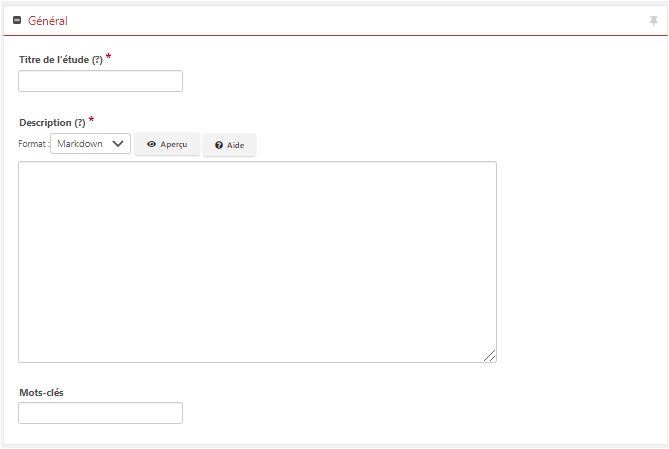
\includegraphics[width=9cm,trim = 0 0 100 0 , clip = true]{pictures/GEA-general.png}\vspace*{0.2cm}
   \captionof{figure}{\label{figure:GEA-general}Constitution d'une fiche de Suivi d'Etude - partie générale}

\end{minipage}

\vspace{0.5cm}

\begin{minipage}[c]{0.45\linewidth}
\textbf{Contexte}
\begin{itemize}[label=$\Rightarrow$, font=\LARGE]
   \item \textbf{Projet} (\textit{type :} liste de choix) : à renseigner si l'étude est réalisée dans le cadre du financement par un projet
   \item \textbf{Lot/application} (\textit{type :} liste de choix) : spécifie le lot du projet si le champ précédent a été renseigné
   \item \textbf{Accords de confidentialité} (\textit{type :} liste de caractères) : renseigne si l'étude est soumise à des accords de confidentialité et dans quel cadre d'accord
   \item \textbf{Partenariat} (\textit{type :} liste de caractères) : permet de préciser si l'étude a été réalisée en partenariat avec une autre entité (laboratoire, université, partenaire industriel,...)
   \item \textbf{Jalon} (\textit{type :} bouton radio - \textbf{champ obligatoire}) : définit si l'étude constitue un jalon pour un projet
   \item \textbf{Livrable} (\textit{type :} liste de choix - \textbf{champ obligatoire}) : définit si un livrable doit être émis suite à l'étude
   \item \textbf{DR} (\textit{type :} liste de choix - \textbf{champ obligatoire}) : renseigne si l'étude est soumise à une règle restreinte de diffusion
\end{itemize}

\end{minipage} \hfill
\begin{minipage}[c]{0.5\linewidth}
   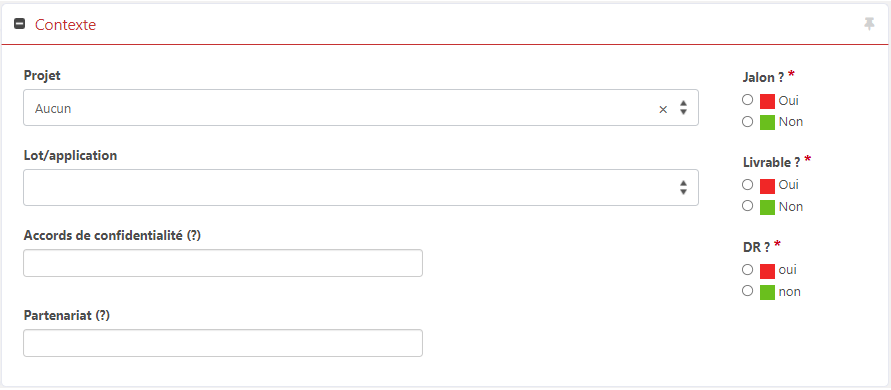
\includegraphics[width=9cm]{pictures/GEA-contexte.png}\vspace*{0.2cm}
   \captionof{figure}{\label{figure:GEA-contexte}Constitution d'une fiche de Suivi d'Etude - partie contexte}

\end{minipage}

\vspace{0.5cm}
\textbf{Informations sur l'étude}
\begin{itemize}[label=$\Rightarrow$, font=\LARGE]
   \item \textbf{Autre personne potentiellement intéressée} (\textit{type :} liste ouverte avec lien vers les membres du projet) : permet de retrouver dans l'annuaire du Tracker, les personnes potentiellement intéressées/concernées par la fiche. Toute personne stipulée dans ce champ recevra un e-mail automatique du BugTracker la renseignant sur les modifications apportées dans la fiche.
   \item \textbf{Catégorie} (\textit{type :} case à cocher) : permet d'identifier si il s'agit d'une nouvelle étude, de la reprise d'une étude,...
\end{itemize}

\begin{minipage}[c]{0.45\linewidth}
\begin{itemize}[label=$\Rightarrow$, font=\LARGE]
   \item \textbf{Version} (\textit{type :} liste de choix) : renseigne sur la version du code utilisée pour mener l'étude. Les différentes versions livrées depuis la v1.7.9 sont disponibles dans le menu déroulant ainsi que la version de développement. Si l'étude était menée sur la version de développement, il est indispensable de renseigner le champ suivant.
   \item \textbf{Préciser SHAI-ID si version développement ou autre version} (\textit{type :} chaîne de caractères) : correspond au "code barre" ou SHA1 ID sous le gestionnaire de configuration GIT, de la version de développement utilisée pour mener l'étude.
\end{itemize}

\end{minipage} \hfill
\begin{minipage}[c]{0.5\linewidth}
   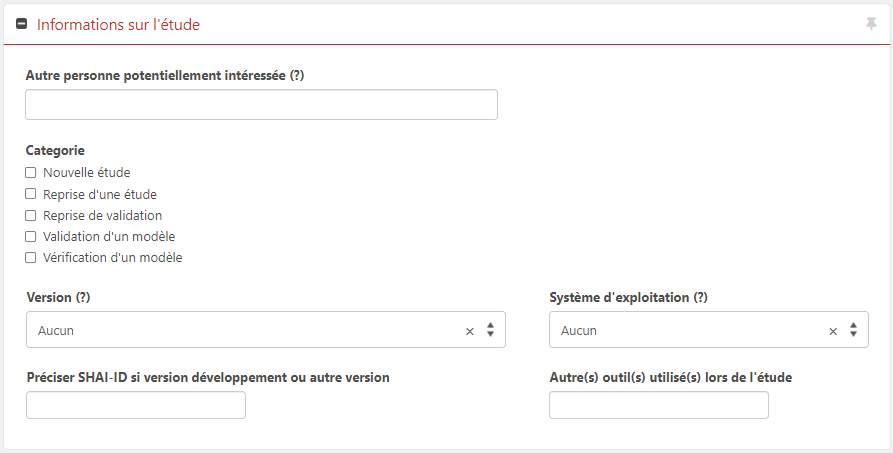
\includegraphics[width=9cm]{pictures/GEA-info.png}\vspace*{0.2cm}
   \captionof{figure}{\label{figure:GEA-info}Constitution d'une fiche de Suivi d'Etude - partie informations sur l'étude}

\end{minipage}

\begin{itemize}[label=$\Rightarrow$, font=\LARGE]
   \item \textbf{Système d'exploitation} (\textit{type :} liste de choix) : renseigne sous quel système d'exploitation l'étude a été menée. En effet, on peut parfois observer de petits écarts de portabilité entre les machines. Si l'étude archivée était amenée à être reprise ou en cas d'inspection des Autorités de Sureté, cette information est capitale.
   \item \textbf{Autre(s) outil(s) utilisé(s) lors de l'étude} (\textit{type :} chaîne de caractères) : si d'autres outils ont été utilisés dans le cadre de l'étude (\textit{eg} SHAPER pour la construction de la CAO, SALOME pour l'établissement du maillage), le ou les outil(s) ainsi que leur version sont à renseigner ici.
\end{itemize}

\vspace{0.5cm}

\begin{minipage}[c]{0.45\linewidth}
\textbf{Avancement}
\begin{itemize}[label=$\Rightarrow$, font=\LARGE]
   \item \textbf{Etat d'avancement} (\textit{type :} liste de choix - \textbf{champs obligatoire}) :  correspond à l'état de vie de la fiche. Cette notion sera plus approfondie dans la section suivante. 
   \item \textbf{Traité par} (\textit{type :} liste à choix multiple avec lien vers les membres du projet) : correspond à(aux) membre(s) du projet travaillant sur le traitement de la DI.
\end{itemize}

\end{minipage} \hfill
\begin{minipage}[c]{0.5\linewidth}
   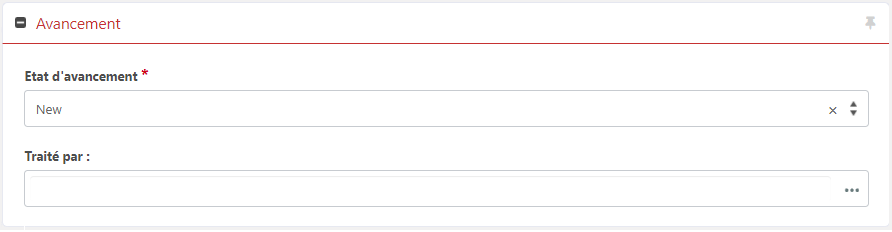
\includegraphics[width=9cm]{pictures/GEA-avancement.png}\vspace*{0.2cm}
   \captionof{figure}{\label{figure:GEA-avancement}Constitution d'une fiche de Suivi d'Etude - partie avancement de l'étude}

\end{minipage}

\vspace{0.5cm}

\textbf{Finalisation de l'étude}\\
Cette partie est à renseigner lorsque l'étude est terminée.
\begin{itemize}[label=$\Rightarrow$, font=\LARGE]
   \item \textbf{Données finales sauvegardées sur Titania} (\textit{type :} cases à cocher) :  correspond à la liste des données qui auront été sauvegardées sur Titania. Ainsi, à la consultation d'une fiche, l'utilisateur saura immédiatement quelles données pourront être accessibles rapidement puisque sauvegardées sur le système d'archivage des études.
   \item \textbf{Autres données sauvegardées sur Titania} (\textit{type :} chaîne de caractères) : si d'autres données ont été sauvegardées sur Titania mais ne correspondent pas aux catégories proposées dans le champ précédent, elles peuvent être renseignées manuellement dans celui-ci.
\end{itemize}
\begin{minipage}[c]{0.45\linewidth}

\begin{itemize}[label=$\Rightarrow$, font=\LARGE]
   \item \textbf{Référence note émise} (\textit{type :} chaîne de caractères) : si dans le cadre de cette étude, une note a été émise, il est possible d'en renseigner son numéro d'émission ici afin de la retrouver plus rapidement dans la base documentaire de notes du département.
   \item \textbf{Temps passé (jours)} (\textit{type :} chaîne de caractères) : peut être rempli pour donner un retour d'expérience sur le temps nécessaire pour traiter chaque catégorie d'étude et faciliter les chiffrages postérieurs.
\end{itemize}

\end{minipage} \hfill
\begin{minipage}[c]{0.5\linewidth}
   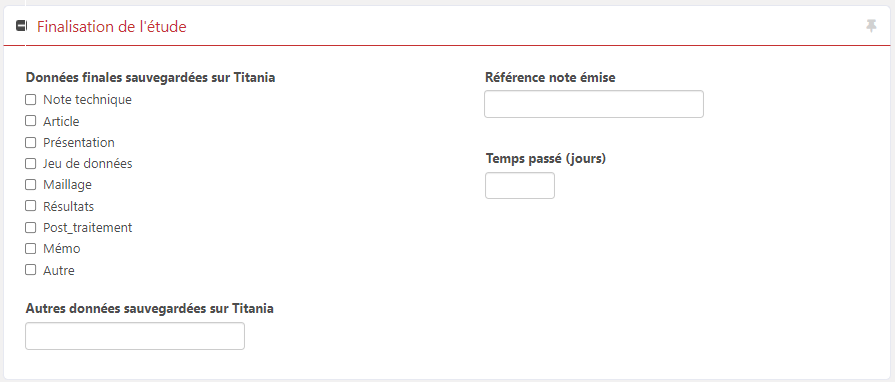
\includegraphics[width=9cm]{pictures/GEA-finalisation.png}\vspace*{0.2cm}
   \captionof{figure}{\label{figure:GEA-finalisation}Constitution d'une fiche de Suivi d'Etude - partie finalisation de l'étude}

\end{minipage}

\vspace{0.5cm}

\begin{minipage}[c]{0.45\linewidth}
\textbf{Pièces jointes}\\
Des données légères peuvent être sauvegardées ici mais il ne s'agit, en aucun cas du lieu d'archivage de l'étude. Tuleap n'est pas conçu pour supporter de gros volumes de données et au delà de 50 Go de données stockées, son temps de réponse devient très important, nuisant fortement à son utilisation. Ainsi, seules des données de petites tailles (\textit{eg} échanges de mail, supports de présentation,...) peuvent être sauvegardées ici. Ces données correspondent plutôt à des données nécessaires lors de l'étude et devront ensuite être sauvegardées sur le système d'archivage.\\
\end{minipage} \hfill
\begin{minipage}[c]{0.5\linewidth}
   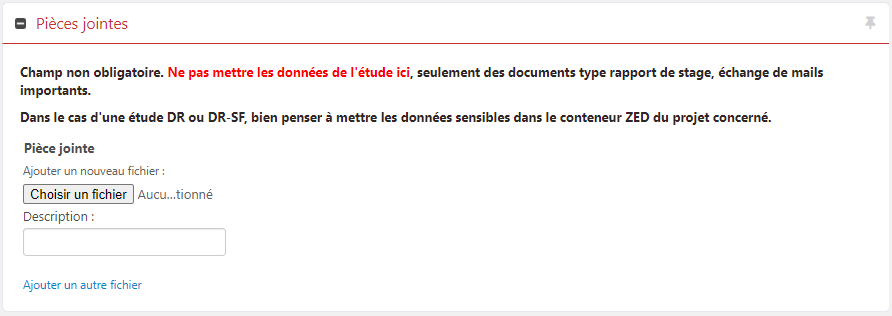
\includegraphics[width=9cm]{pictures/GEA-PJ.png}\vspace*{0.2cm}
   \captionof{figure}{\label{figure:GEA-PJ}Constitution d'une fiche de Suivi d'Etude - partie pièces jointes}

\end{minipage}

D'autre part, en cas d'une étude contenant des données sensibles (type Diffusion Restreinte ou Diffusion Restreinte - Spéciale France), ces données ne devront pas figurer "en clair" dans la fiche de Suivi de l'Etude. Elles devront avoir été préalablement placées dans le conteneur du projet hébergeant l'étude. C'est ce conteneur qui sera ensuite sauvegardé en pièce jointe dans la fiche.

\vspace{0.5cm}

\begin{minipage}[c]{0.45\linewidth}
\textbf{Permissions}\\
Le dernier champ a remplir avant la finalisation de la fiche de Suivi d'Etude concerne les droits d'accès à celle-ci. Ce champ est \textbf{obligatoire}. Si il s'agit d'une étude contenant des données sensibles (type Diffusion Restreinte ou Diffusion Restreinte - Spéciale France), il faudra veiller à sélectionner uniquement le groupe DRSF-STMF. Seul ce groupe-là pourra alors voir les études de ce type. Pour les autres études n'ayant aucune donnée sensible, le groupe Permanents-STMF sera à sélectionner ainsi que le groupe temporaires-STMF si on souhaite mettre la fiche à disposition des personnes n'étant pas en contrat permanents (stagiaires, doctorants, post-doc, CDD,...). \\
\end{minipage} \hfill
\begin{minipage}[c]{0.5\linewidth}
   \begin{figure}[H]
      \centering
      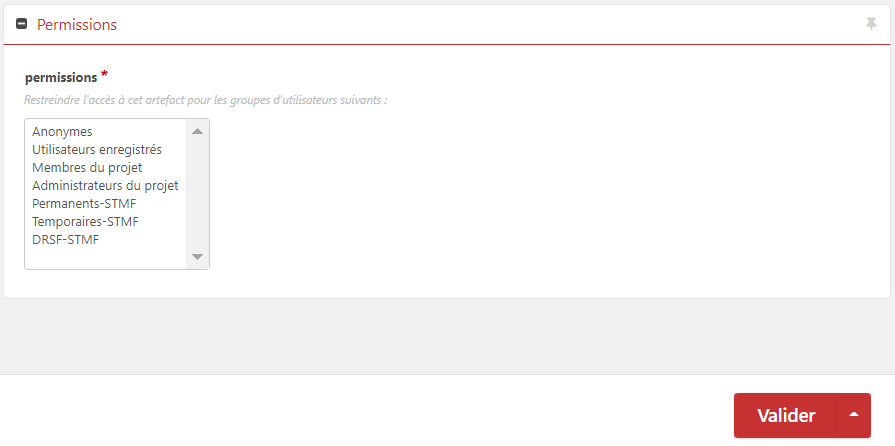
\includegraphics[width=9cm]{pictures/GEA-permissions.png}
      \vspace*{0.2cm}
      \captionof{figure}{\label{figure:GEA-permissions}Constitution d'une fiche de Suivi d'Etude - partie permissions}
   \end{figure}
\end{minipage}

Lorsque tous les champs ont bien été remplis, veillez à bien appuyer sur le bouton \texttt{Valider} afin de générer la création de la fiche. L'ensemble des champs peut être modifié après la création de la fiche.

\vspace{0.5cm}

\begin{minipage}[c]{0.5\linewidth}
   \begin{figure}[H]
      \centering
      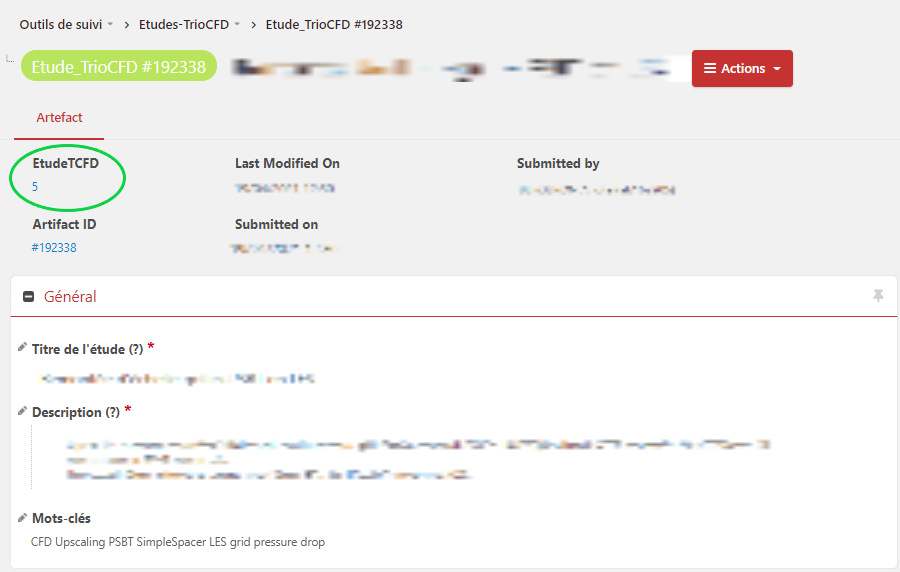
\includegraphics[width=8cm]{pictures/GEA-identification.png}
      \vspace*{0.2cm}
      \captionof{figure}{\label{figure:GEA-identification}Constitution d'une fiche de Suivi d'Etude - numéro d'identification de la fiche}
   \end{figure}
\end{minipage} \hfill
\begin{minipage}[c]{0.45\linewidth}
Une fois la fiche créée, elle dispose alors d'un identifiant unique (voir encadré vert sur figure ci-contre). Cet identifiant servira à nommer le répertoire de sauvegarde de l'étude afin de le retrouver immédiatement sur le système d'archivage sous Titania.

\end{minipage}


\subsection{États de traitement d'une fiche de suivi d'étude}

Contrairement au BugTracker informatique, le gestionnaire de suivi des études comporte un Worflow beaucoup plus simple avec seulement 4 états pour une fiche de Suivi d'Etude. Ces 4 états sont les suivants :
\begin{itemize}[label=$\Rightarrow$, font=\LARGE]
   \item \textbf{NEW} : à la création de la fiche de Suivi d'Etude, celle-ci est automatiquement en statut NEW. L'étude a été identifiée mais le travail dessus n'a pas encore été amorcé.
   \item \textbf{IN PROGRESS} : dès que le travail est amorcé, la personne en charge de l'étude passe la fiche de suivi correspondante à l'état IN PROGRESS. Pour le passage dans ce statut, il est nécessaire de renseigner le champ \texttt{Traité par}. En effet, à ce stade, il y a nécessairement une personne qui a été identifiée pour mener à bien cette étude. La fiche de Suivi de l'Etude va passer la majorité de sa vie dans cet état.
   \item \textbf{SAVED} : une fois l'étude, à proprement parler, terminée, les données nécessaires à sa reproduction ou reprise doivent être archivée sur le système d'archivage sous Titania. Une fois que cet archivage est fait, la fiche passe alors en statut SAVED. Pour ce passage, 2 champs de la fiche doivent avoir été au préalablement remplis à savoir \texttt{Données sauvegardées sur Titania} et \texttt{Version}. Ce dernier champ est, en effet, absolument nécessaire pour que les données archivées puissent être ré-exploitées. Un jeu de données peut différer d'une version à l'autre du code mais également être fonctionnel sur des versions antérieures et, nécessiter une mise à jour pour qu'il le soit sur une nouvelle version.
   \item \textbf{CLOSED} : une fois l'étude menée et les documents associés archivés, la fiche de suivi peut alors être clôturée.
\end{itemize}

Il s'agit là du déroulé le plus standard d'une fiche d'étude. Il est toutefois possible qu'il y ait plusieurs itérations avant qu'une fiche ne soit clôturée. La figure \ref{figure:worflow-etude} représente l'ensemble du Worflow et récapitule les champs nécessaires pour le passage d'un statut à l'autre.\\
\vspace{0.1cm}
\begin{figure}[H]
   \centering
   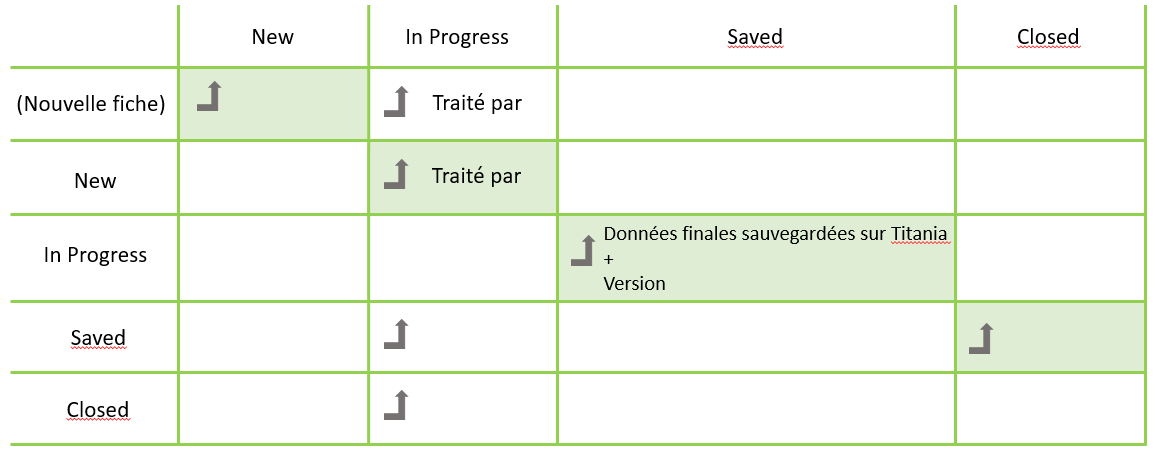
\includegraphics[width=13cm]{pictures/worflow-etude.png}                        
   \vspace*{0.2cm}
   \captionof{figure}{\label{figure:worflow-etude}Worflow du gestionnaire de suivi des études de TrioCFD}
\end{figure}
\subsection{Archivage des études}
Avant de passer dans l'état SAVED décrit au paragraphe précédent, toutes les données nécessaires à la reprise de l'étude doivent avoir été archivée sur Titania. Cette méthodologie d'archivage va être décrite dans cette section.\\

Le système d'archivage Linux est présent sur le nouveau système Linux du DM2S nommé Titania. Il est accessible autant depuis Linux que depuis Windows. Celui-ci s'appelle etudes-stmf (même nom que le projet sur Tuleap, moyennant la casse). L'accès à l'espace de stockage via LINUX se fait à partir d'un poste connecté à Titania. L'espace est ensuite accessible sur /home/etudes-stmf :
\begin{lstlisting}
> cd /home/etudes-stmf 
\end{lstlisting}
On trouve ici les répertoires des différents codes participant au projet, donc TrioCFD, et présents sur le gestionnaire d'études dans Tuelap.\\
Pour avoir accès à l'espace d'archivage via Windows, il suffit d'ouvrir un explorateur de fichier et de saisir l'adresse suivante dans la barre d'accès en haut de la fenêtre :
\begin{lstlisting}
\\titania\home_projet\partage/etudes-stmf
\end{lstlisting}
Il est conseillé de connecter un lecteur sur cet emplacement afin de ne pas avoir à le rechercher à chaque fois. Comme sur Linux, vous aurez alors accès aux répertoires des différents codes participant au projet et présents sur le gestionnaire d'études dans Tuleap (voir figure \ref{figure:Sauvegarde-Titania}).\\
Sous chacun des répertoires des codes, autant de répertoires que de fiches de Suivi d'Etude présentes sur Tuleap devront être créés. A un répertoire correspond les données d'une fiche d'étude. Le lien entre la fiche étude sous Tuleap et le répertoire d'archivage sur Linux se fera via le nom donné au répertoire sur le système d'archivage qui correspondra au numéro de l'étude généré par Tuleap. Chaque répertoire d'étude est composé de plusieurs sous-dossiers avec une structure identique pour chaque étude :
\begin{itemize}[label=$\Rightarrow$, font=\LARGE]
   \item \textbf{01-MEMO} : un ou plusieurs mémos permettant de bien identifier les données qui ont été archivées comme l'organisation des répertoires de calculs ou toute information qui semble utile pour permettre la bonne compréhension et reproductibilité de l'étude.
   \item \textbf{02-Donnees\_Entrees} : ce répertoire a pour but de stocker les données qui ont été nécessaires à la modélisation de l'étude (plans de l'expérience si une comparaison par rapport à l'expérimental a été faite, le jdd d'origine si il s'agit d'une reprise d'étude,...) 
   \item \textbf{03-Calculs} : c'est ici que sont stockés l'ensemble des jdds, maillages, post-traitement et éventuellement les résultats. Il se peut que de nombreux jdds aient été créés pour mener à bien l'étude. Il est recommandé de procéder, tout d'abord à un tri de ces calculs puis de ranger chacun d'entre eux dans un répertoire différent sous 03-Calculs par exemple Calcul01, Calcul02,... (nommage à la discrétion de chacun). Chaque répertoire de calcul contiendra le maillage propre au calcul, le jdd, le fichier de post-traitement et éventuellement, les résultats. Afin de mieux comprendre en quoi consiste chacun de ces répertoires de calcul une fiche mémo pourra être élaborée et sauvegardée dans \texttt{01-MEMO}
   \item \textbf{04-Documents\_Emis} : seront sauvegardés ici tous les documents émis suite à cette étude. Cela pour être un article, une présentation, une note technique,... 
   \item \textbf{05-Verification} : seront sauvegardés dans ce répertoire tous les retours et échanges qui auraient pu y avoir dans le cadre de la vérification de l'étude
   \item \textbf{06-References} : seront sauvegardés ici les articles ou autres références bibliographiques ayant contribué aux réflexions menées durant l'étude
   \item \textbf{07-Codes-scripts} : si des scripts ou des codes non suivis en gestion de configuration (git, github,...) ont été élaborés dans le cadre de l'étude, ils seront stockés dans ce sous-répertoire.
\end{itemize}
\begin{figure}[H]
   \centering
   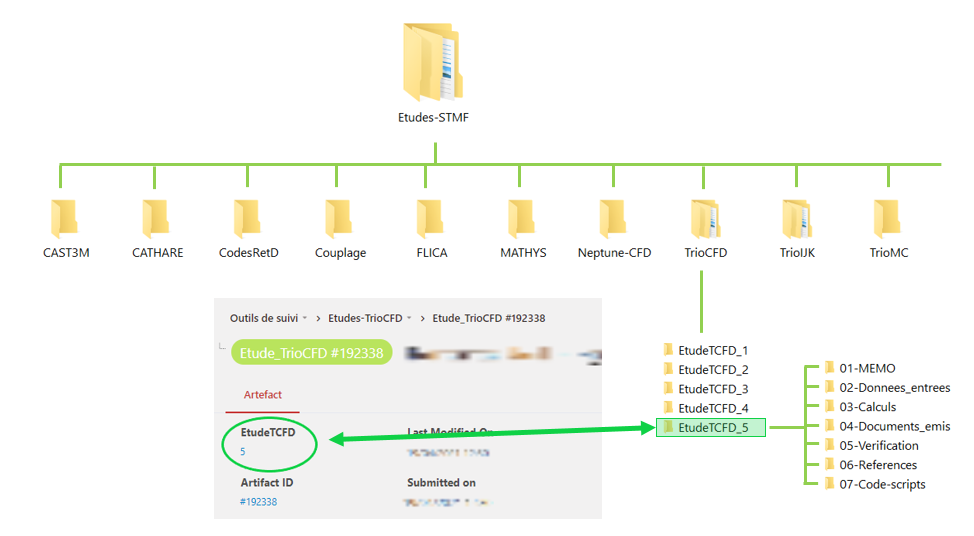
\includegraphics[width=14.5cm]{pictures/Sauvegarde-Titania.png}
   \vspace*{0.2cm}
   \captionof{figure}{\label{figure:Sauvegarde-Titania}Organisation de la sauvegarde des études sous Titania}
\end{figure}
\vspace{0.2cm}
Afin de générer rapidement cette arborescence, un script est présent dans le répertoire de TrioCFD. Celui-ci ce nomme \texttt{gen\_dossier.sh}. Il est alors demandé le numéro de la fiche pour laquelle le dossier doit être créé et l'ensemble est alors automatiquement généré. Son déroulé a lieu de la façon suivante (exemple de la figure \ref{figure:Sauvegarde-Titania}):

\footnotesize
\begin{lstlisting}
 > ./gen_dossier.sh             % lancement script
 Numero de la fiche Tuleap ?    % demande du numero de la fiche Tuleap correspondante
 5                              % numero renseigne par l'utilisateur
 Repertoire EtudeTCFD_5 cree    % message de succes de la creation
\end{lstlisting}
\normalsize
Le remplissage de tous les répertoires présentés ci-dessus n'est, en aucun cas, obligatoire tant que toutes les données indispensables à la compréhension et la reproductibilité de l'étude sont présentes. Si un répertoire est vide, il est demandé de ne pas le supprimer et le laisser vide, en l'état.\\
Pour le stockage des documents, les formats de stockage des données doivent être les plus standard possibles et lisibles par une majorité d'OS à savoir des fichiers texte (jeux de données, post-traitement, scripts, latex,...) ou des fichiers pdf. En cas de  sauvegarde de fichiers à format propriétaire, type Office ou LibreOffice, il est recommandé d'archiver à la fois ce type de fichier mais également leur impression au format pdf.\\
\\
L'ensemble de cette méthodologie pour le suivi et l'archivage d'une étude est détaillé dans le MediaWiki du projet Tuleap Etudes-STMF à l'adresse : \url{https://codev-tuleap.intra.cea.fr/plugins/mediawiki/wiki/etudes-stmf/index.php?title=Accueil}.

\chapter{\label{chapitre:GIT}Outil de gestion de versions (GIT)}
\lhead{Outil de gestion de versions}
\rhead{OUTILS}
Deux ans après le début du développement de la plateforme, celle-ci est passée en gestion de configuration, d'abord sous SCCS, puis sur ClearCase et depuis mi 2013 sur GIT. L'ensemble du code TrioCFD y est stocké que ce soit le code source, les procédures, les fiches de V\&V ou la documentation. Cette base GIT est hébergée par Tuleap et se nomme triocfd-code.\\
\\
\subsection{Définition de la gestion de versions}
Le contrôle de version, également appelé contrôle de source, désigne la pratique consistant à suivre et à gérer les changements apportés au code d'un logiciel. Les systèmes de contrôle de version sont des outils logiciels qui permettent aux équipes de développement de gérer les changements apportés au code source au fil du temps. Les logiciels de contrôle de version gardent une trace de chaque changement apporté au code dans un type spécial de base de données. Si une erreur est commise, les développeurs peuvent revenir en arrière et comparer les versions antérieures du code, ce qui leur permet de corriger l'erreur tout en minimisant les perturbations pour tous les membres de l'équipe. 
Les développeurs qui travaillent en équipe écrivent continuellement du nouveau code source et modifient le code source existant. Le code d'un projet logiciel est généralement organisé en une structure de dossiers ou « arborescence de fichiers ». Un développeur de l'équipe peut travailler sur une nouvelle fonctionnalité, tandis qu'un autre corrige un bug sans rapport en changeant le code. Chaque développeur peut apporter ses changements dans plusieurs parties de l'arborescence de fichiers.\\
Le contrôle de version aide les équipes à résoudre ce genre de problèmes, en suivant chaque changement individuel de chaque contributeur et en aidant à prévenir les conflits entre les tâches concomitantes. Les changements apportés à une partie du logiciel peuvent être incompatibles avec ceux apportés par un autre développeur travaillant en même temps. Ce type de problème doit être identifié et résolu de manière ordonnée sans bloquer le travail du reste de l'équipe. En outre, dans tout projet de développement, le moindre changement peut introduire de nouveaux bugs, et la nouvelle version du code ne peut être considéré comme fiable tant qu'elle n'a pas été testée. Les tests et le développement se poursuivent donc en parallèle jusqu'à ce qu'une nouvelle version soit prête.\\
Les principaux avantages du contrôle de version sont les suivants :
\begin{itemize}
   \item \textbf{Un historique complet des changements à long terme de chaque fichier} : le moindre changement effectué par de nombreuses personnes au fil des ans. Les changements comprennent la création et la suppression de fichiers, ainsi que l'édition de leur contenu. Cet historique doit également comprendre l'auteur, la date et des notes écrites sur l'objet de chaque changement. Le fait de disposer de l'historique complet permet de revenir aux versions précédentes pour aider à l'analyse des causes profondes des bugs, ce qui est crucial lorsqu'il est question de corriger des problèmes dans les anciennes versions d'un logiciel.
   \item \textbf{Branching et merges} : Le fait que les membres d'une équipe travaillent simultanément est une évidence, mais il peut être intéressant pour les personnes autonomes de pouvoir travailler sur des flux de changements indépendants. La création d'une « branche »  permet de garder plusieurs flux de travail indépendants les uns des autres, tout en offrant la possibilité de fusionner ces tâches, permettant ainsi aux développeurs de vérifier que les changements sur les différentes branches n'entrent pas en conflit.
   \item \textbf{Traçabilité} : Pouvoir retracer chaque changement apporté au logiciel et le connecter à des logiciels de gestion de projet et de suivi des BugTracker comme Tuleap, et être capable d'annoter chaque changement avec un message décrivant son but peut contribuer à l'analyse des causes profondes d'un bug. Avoir sous la main l'historique annoté du code pendant sa lecture, essayer de comprendre ce qu'il fait et pourquoi il est ainsi conçu, peut permettre aux développeurs d'apporter des changements appropriés et harmonieux, en accord avec l'architecture prévue du système. Cela peut être particulièrement important pour travailler efficacement avec le code existant et pour permettre aux développeurs d'estimer les futures tâches avec précision.
\end{itemize}
\subsection{Logiciel actuel de gestion de versions de TrioCFD : GIT}
GIT est un logiciel de gestion de versions décentralisé.
Le code informatique développé est stocké non seulement sur l'ordinateur de chaque contributeur du projet, mais également sur le serveur dédié. Il s'agit d'un outil de bas niveau, qui se veut simple et performant et dont la principale tâche est de gérer l'évolution du contenu d'une arborescence. GIT indexe les fichiers d'après leur somme de contrôle calculée avec la fonction de hachage SHA1 ID. Quand un fichier n'est pas modifié, la somme de contrôle ne change pas et le fichier n'est stocké qu'une seule fois. En revanche, si le fichier est modifié, les deux versions sont stockées sur le disque. Le SHA1 ID protège le code et l'historique des changements contre toute modification accidentelle ou malveillante, tout en assurant une traçabilité complète de l'historique. GIT prend en charge le branching et le tagging en priorité et les opérations qui concernent les branches et les tags (comme les merges et les reverts) sont également stockées dans l'historique des changements. GIT présente également une très grande flexibilité et est capable de prendre en charge le workflow propre à chaque projet. Celui de TrioCFD est décrit dans la section suivante.

\subsection{\label{subsec:WorkflowGIT}Organisation générale et Workflow de TrioCFD sur GIT}
Pour chaque modification, correction ou développement dans le code, que cela concerne les sources à proprement parler mais également la documentation, les cas tests ou les procédures,  une fiche de Demande d'Intervention (voir chapitre \ref{chapitre:tracker-info}) doit être créée. Une branche correspondante sera, à son tour, créée sous GIT. La méthodologie 1 problème = 1 DI = 1 branche permet d'assurer un excellent suivi de tout changement fait dans le code et de pouvoir reconstruire une version du code pour chacun d'eux.\\
Après avoir créé la fiche de Demande d'Intervention, le déroulé sous GIT est le suivant :
\begin{enumerate}
   \item \textbf{Définition du nom de la branche de travail} - assuré par le développeur : le nom de la branche dans laquelle le travail va être réalisé devra porter le formalisme suivant : TCFDXXXXXX\_ACTIVITE où XXXXXX correspondra à l' "Artifact ID" (numéro d'identification) de la fiche qui a été créé suivant la méthodologie   décrite dans la section \ref{subsec: ficheDI} et ACTIVITE, l'activité sur laquelle porte la branche.
   \item \textbf{Création de la branche sur le dépôt GIT local} - assuré par le développeur : à partir du dépôt local de TrioCFD, le développeur crée sa branche à partir de la version en développement du code (branche triou/TMA) : 
   \begin{lstlisting}
   > git checkout -b TCFDXXXXXX_ACTIVITE origin/triou/TMA
   \end{lstlisting}
   En lançant ensuite la commande git \texttt{git branch} , le développeur s'assurera que la branche TCFDXXXXXX\_ACTIVITE a bien été créée sur son dépôt local.
   \item \textbf{Sauvegarde régulière de la branche de travail} - assurée par le développeur : après avoir effectué une partie de son développement (voir chapitre \ref{chapter:dev} décrivant le processus de développement et sa structuration), le développeur effectue une sauvegarde de son travail sur le dépôt GIT distant. Il doit, au préalable s'être assuré que le code compilait correctement et que la base de vérification avait tourné avec succès. La sauvegarde se fait via un point de commit et la branche de développement est ensuite publiée sur le dépôt distant de TrioCFD :
   \footnotesize
   \begin{lstlisting}
   > git add <path/to/fileName>           % ajout des fichiers voulant etre sauvegardes
   > git commit                           % creation d'un point de commit
   > git push origin TCFDXXXXXX_ACTIVITE  % envoi de la branche sur le depot distant
   \end{lstlisting}
   \normalsize
   Cette étape sera répétée autant de fois que nécessaire jusqu'à ce que les actions menées dans le cadre de cette Demande d'Intervention soient considérées comme finies. 
   \item \textbf{Demande de Pull Request} - assuré par le développeur : une fois l'ensemble des commits réalisés sur la branche TCFDXXXXXX\_ACTIVITE ainsi que les vérifications de bonne compilation du code et du bon déroulé de la base de vérification, le développeur informe le Responsable de Code que sa branche est prête à être intégrée dans TrioCFD via une Pull Request de sa branche vers la branche triou/TMA (voir Figure \ref{figure:tuleap_PR})
   \item \textbf{Relecture de la branche de développement} - assurée par le relecteur : le Responsable de Code demande à un des relecteurs de l'équipe de développement de TrioCFD de procéder à la relecture de la branche (voir la section \ref{subsec:relecture}). Il s'assure du bon respect des règles de méthodologie et de codage dans la branche TCFDXXXXXX\_ACTIVITE. Il itère autant de fois que nécessaires avec le développeur afin que la branche soit propre et fonctionnelle. Suite à la relecture, le développeur peut être amené à effectuer des modifications afin que sa branche atteigne un niveau de conformité satisfaisant. Une fois cet objectif atteint, il appose le tag \texttt{OK pour intégration} au niveau de la Pull Request.
   \item \textbf{Intégration de la branche de développement} - assurée par l'intégrateur : une fois la relecture achevée avec succès, l'intégrateur prend en charge son intégration dans la branche en développement de TrioCFD. Il commence par fusionner la branche de développement (TCFDXXXXXX\_ACTIVITE) avec la branche en développement de TrioCFD (triou/TMA) via un \texttt{git merge}. En cas de conflits entre elles, il s'occupe de leur résolution en faisant appel, si nécessaire, au développeur. Si cette fusion n'entraîne aucun conflit, il compile cette nouvelle version obtenue par la fusion et lance une base de vérification. En cas de problème sur la base de vérification, il se tourne vers le développeur pour que celui-ci résolve les problèmes observés. Si la base de vérification passe sans difficulté et qu'aucun impact n'est prévu suite à la branche de développement, il entérine la fusion des 2 branches et envoie sur le dépôt distant la nouvelle version de la branche \texttt{triou/TMA} via la commande \texttt{git push}. Si des impacts sont à prévoir sur la base de Validation du code, celle-ci est lancée et les impacts observés, validés, avant que le développement ne soit intégré dans \texttt{triou/TMA}.
\end{enumerate} 
Le Worflow sous GIT, décrit ci-dessus, est illustré en Figure \ref{figure:workflow_GIT}.
\begin{figure}[H]
   \centering
   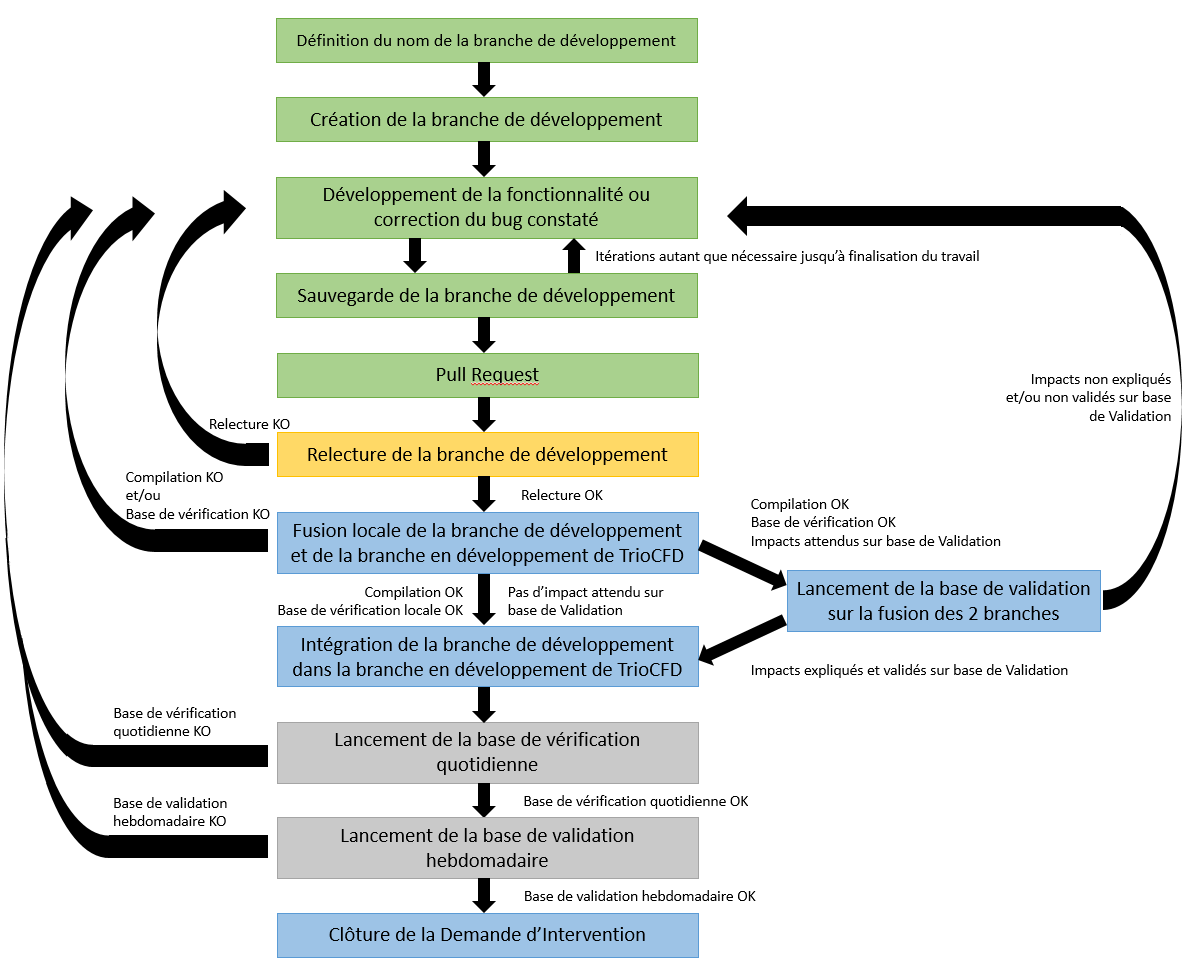
\includegraphics[width=16cm]{pictures/workflow_GIT.png}
   \vspace*{0.2cm}
   \captionof{figure}{\label{figure:workflow_GIT}Worflow de TrioCFD sous GIT pour une branche de développement - en vert : tâches développeur - en jaune : tâche relecteur - en bleu : tâche intégrateur - en gris : tâches Atelier Logiciel}
\end{figure}
\vspace{0.2cm}
En plus de garantir une bonne traçabilité pour tout changement apporté dans le code, cette méthodologie permet d'avoir une lecture facilitée de la base GIT du code. Quand cette méthodologie est étendue à tous les développements en cours sur le code, le flux sur GIT pour TrioCFD peut être illustré par la figure \ref{figure:workflow_GIT2}. L'ensemble de cette méthodologie est décrite sur le MediaWiki du projet TrioCFD sur Tuleap (\url{https://codev-tuleap.intra.cea.fr/plugins/mediawiki/wiki/triocfd/index.php?title=Accueil})\vspace{0.5cm}\\

La branche \texttt{triou/TMA} correspond donc à la version en développement de TrioCFD qui évolue au gré des intégrations en continu dans le code et sur laquelle tous les développeurs du code CEA doivent travailler. La branche \texttt{master}, quant à elle, est mise à jour à chaque sortie de version et correspond à la dernière version livrée du code. A la mise à jour de la branche \texttt{master} pour la sortie de version, un tag est également apposé et nommé suivant le numéro de la version livrée.\\
\begin{figure}[H]
   \centering
   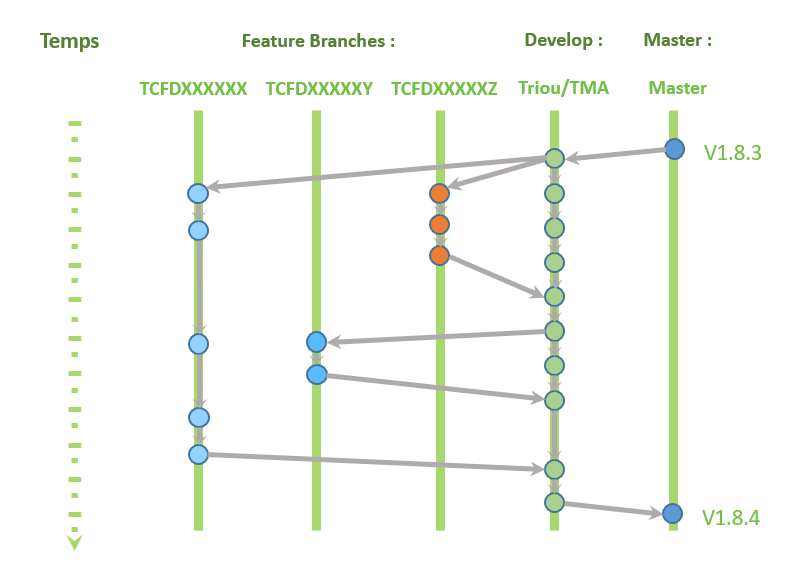
\includegraphics[width=16cm]{pictures/workflow_GIT2.png}
   \vspace*{0.2cm}
   \captionof{figure}{\label{figure:workflow_GIT2}Worflow général de TrioCFD sous GIT}
\end{figure}
\vspace{0.2cm}
La branche \texttt{triou/TMA} est mise à jour quotidiennement par l'Atelier de Génie Logiciel sur le dépôt extérieur de TrioCFD hébergé sur GITHUB à cette adresse : \url{https://github.com/cea-trust-platform/TrioCFD-code}. Ce dépôt extérieur permet aux développeurs hors CEA de travailler de la même façon que les développeurs CEA avec une version en développement du code à jour, nommée \texttt{next} sur GITHUB. Pour ce faire, ils créent également une \texttt{Issue} (qui est l'équivalent d'une Demande d'Intervention sur Tuleap) et nomment leur branche, en fonction, sous GITHUB. Afin de centraliser sur un seul Tracker l'ensemble des actions concernant TrioCFD, le Responsable de Code aura la charge de basculer l'ensemble des données présentes sur GITHUB sur Tuleap et renommer la branche de GITHUB en conséquence sur GIT avant son intégration dans le code.
\chapter{\label{chapitre:messagerie}Messagerie}
\lhead{Messagerie}
\rhead{OUTILS}

Afin d'échanger avec la TMA, une adresse de messagerie est \`a disposition des utilisateurs : \href{mailto:trust@cea.fr}{trust@cea.fr}. Cette adresse est exclusivement g\'er\'ee par la TMA.\\
Il s'agit de l'unique moyen de contact entre les utilisateurs du code et l'équipe de TMA. L'adresse personnelle des agents TMA n'est pas utilisée dans le cadre du projet. Cette boîte unique permet de conserver un historique complet des échanges de la TMA avec les utilisateurs. Chaque membre de l'équipe TMA a les droits en lecture et écriture sur cette messagerie.\\
Elle est utilisée pour répondre aux questionnements des utilisateurs mais également pour communiquer des informations pratiques pour les sessions de formations par exemple. Le délai contractuel de traitement des mails re\c cus via cette adresse par l'équipe TMA est d'un jour ouvré. Il est donc fortement recommandé de passer exclusivement par ce biais pour contacter le support (cela n'empêche cependant pas de mettre en copie le RPL ou le Responsable de Code) afin de garantir la bonne tra\c cabilité des échanges et d'être également assuré d'avoir un retour dans les plus brefs délais.


%\chapter{G\'en\'eration de la documentation}
%\lhead{G\'en\'eration de la documentation}
%\rhead{OUTILS}
%\newpage

\chapter{Interfa\c cage pour l'utilisateur et le d\'eveloppeur}
\lhead{Interfa\c cage pour l'utilisateur et le d\'eveloppeur}
\rhead{OUTILS}
Plusieurs scripts et outils sont à la disposition des utilisateurs afin de faciliter l'utilisation de la plateforme TRUST/TrioCFD. Une procédure est dédiée à chaque action effectuée sur la plateforme. Ces outils étant nombreux, ils n'ont pas pu tous être détaillés pour la première version de ce document mais cette partie sera étayée au fil des différentes versions.

\subsection{Trouver la version de TRUST \`a utiliser avec TrioCFD}
\label{subsec:versionTRUST}

Une version donn\'ee de TrioCFD doit \^etre utilis\'ee avec une version sp\'ecifique de TRUST.\\

Le fichier "\emph{./src/Version\_info}" fournit cette version de TRUST sous la forme du "Id SHA1" de git.\\

Par cons\'equent, la premi\`ere chose \`a faire avant de compiler TrioCFD est de se placer (et de compiler)
sur la version associ\'ee de TRUST.\\

Si le "Id SHA1" est par exemple "9296ac998a9b2c6187067b8e5a219dcb814fbb4d", il convient de faire :
\begin{lstlisting}
> cd trust-code
> git checkout 9296ac998a9b2c6187067b8e5a219dcb814fbb4d
> ./configure && make
\end{lstlisting}

\subsection{Installation et compilation de TrioCFD}
\label{subsec:install}

On consid\`ere que la version de TRUST associ\`ee \`a celle de TrioCFD est \`a disposition
(c'est le cas pour les versions officielles par exemple, la version 1.9.2 de TrioCFD
doit s'utiliser avec la version 1.9.2 de TRUST).\\

On commence par charger l'environnement de TRUST de cette version :
\begin{lstlisting}
> source trust-code/env_TRUST.sh
\end{lstlisting}
On configure le passage en mode "Baltik" :
\begin{lstlisting}
> baltik_build_configure
\end{lstlisting}
On lance la configuration de TrioCFD :
\begin{lstlisting}
> ./configure
\end{lstlisting}
On lance la compilation de TrioCFD dans le mode souhaité:
\begin{lstlisting}
> make optim semi-optim debug
\end{lstlisting}

\subsection{Lancement d'un cas test}
Pour lancer un calcul en mode séquentiel, la méthodologie est la suivante :

\begin{lstlisting}
> cd $my_test_directory
> trust my_data_file %whitout .data
\end{lstlisting}

Il s'agit du lancement standard d'un calcul. D'autres options sont disponibles pour effectuer
cette action et sont d\'etaill\`ees ci-apr\`es.
La syntaxe de lancement devient alors :
\begin{lstlisting}
> trust [option] my_data file [nb_cpus] [1>file.out] [2>file.err]
\end{lstlisting}
où \texttt{nb\_cpus} correspond au nombre de processeurs utilisés pour lancer le calcul (ce nombre doit être égal au nombre de sous-domaines définis dans le jeu de données),\\
où les \texttt{options} disponibles sont :

\begin{table}[H]
\begin{centering}
%\scriptsize
\small
\begin{tabular}{Sl Sl}
\hline\hline
\rowcolor{lightgray}\textbf{OPTION} & \textbf{Description} \tabularnewline
\hline
-help | -h & List options \tabularnewline \hline
-baltik & Instanciate an empty Baltik project \tabularnewline \hline
-index & Access to the TRUST ressource index \tabularnewline \hline
-doc & Access to the TRUST manual (Generic Guide) \tabularnewline \hline
-config nedit|vim|emacs|gedit & Configure nedit or vim or emacs with TRUST keywords \tabularnewline \hline
-edit & Edit datafile \tabularnewline \hline
-xedit & Edit datafile with xdata \tabularnewline \hline
-xcheck & Check the datafile’s keywords with xdata \tabularnewline \hline
-partition & Partition the mesh to prepare a parallel calculation \tabularnewline
&(Creation of the .Zones files) \tabularnewline \hline
-mesh & Visualize the mesh(es) contained in the data file \tabularnewline \hline
-probes & Monitor the TRUST calculation only  \tabularnewline \hline
-evol & Monitor the TRUST calculation (new IHM) \tabularnewline \hline
-wiz & Create a TRUST datafile from a MED file (new IHM) \tabularnewline \hline
-prm & Write a prm file \tabularnewline \hline
-clean & Clean the current directory from all the generated
files by TRUST \tabularnewline \hline
-search keywords & Know the list of test cases from the data bases which contain keywords \tabularnewline \hline
-copy & Copy the test case datafile from the TRUST database
under the \tabularnewline
& present directory \tabularnewline \hline
-check all|testcase|list & Check the non regression of all the test cases or a single test case or a list \tabularnewline
& of tests cases specified in a file \tabularnewline \hline
-check function|class|class::method & Check the non regression of a list of tests cases covering a function, \tabularnewline
& a class or a class method\tabularnewline \hline
-gdb & Run under gdb debugger \tabularnewline \hline
-valgrind & Run under valgrind \tabularnewline \hline
-valgrind\_strict & Run under valgrind with no suppressions \tabularnewline \hline
-create\_sub\_file & Create a submission file only \tabularnewline \hline
-prod & Create a submission file and submit the job on the
main production class \tabularnewline 
& with exclusive resource \tabularnewline \hline
datafile -help\_trust & Print options of TRUST\_EXECUTABLE [CASE[.data]] [options] \tabularnewline \hline
\hline
\end{tabular}
\normalsize
\par\end{centering}
\caption{\label{tab:option-cas}Options disponibles pour le lancement d'un cas-test}
\end{table}
